\documentclass[twoside,letterpaper,pdftex]{article}
\usepackage[utf8]{inputenc}
\usepackage{amsmath}
\usepackage{amsfonts}
\usepackage{amssymb}
\usepackage{graphicx}
\usepackage{tabularx}
\usepackage[final]{pdfpages}
\setboolean{@twoside}{false}
\parskip=0pt
\usepackage[left=1in,right=1in,top=1in,bottom=1in]{geometry}
\title{ 
\center
\includegraphics[width=\linewidth]{UIGraphic}\\
		\center\textbf{\Large{Swords and Sorcery Computer Adaptation Documentation}\\
		An overview of requirements, design, implementation, testing and metrics} \\
		Version 1.0}
\author{Prepared by:\\University of Idaho Computer Science 383 Class, Spring 2014\\
\bigskip\\
Prepared for:\\
Dr. Clinton Jeffery\\} 
\date{\today} 
\begin{document}
\maketitle
\pagebreak

\section*{Introduction and Document Description}
This is a collection of the documentation gathered for the computer adaptation of the board game, Swords and Sorcery. The software and system for the computer adaptation of S\&S was implemented in Software Engineering, Spring of 2014, at the University of Idaho. Included are the following documents, in their entirety:
\begin{itemize}
\item Systems and Software Requirements Specification
\item System and Software Design Description
\item Implementation Description
\item Testing Description
\item Metrics Description
\end{itemize}

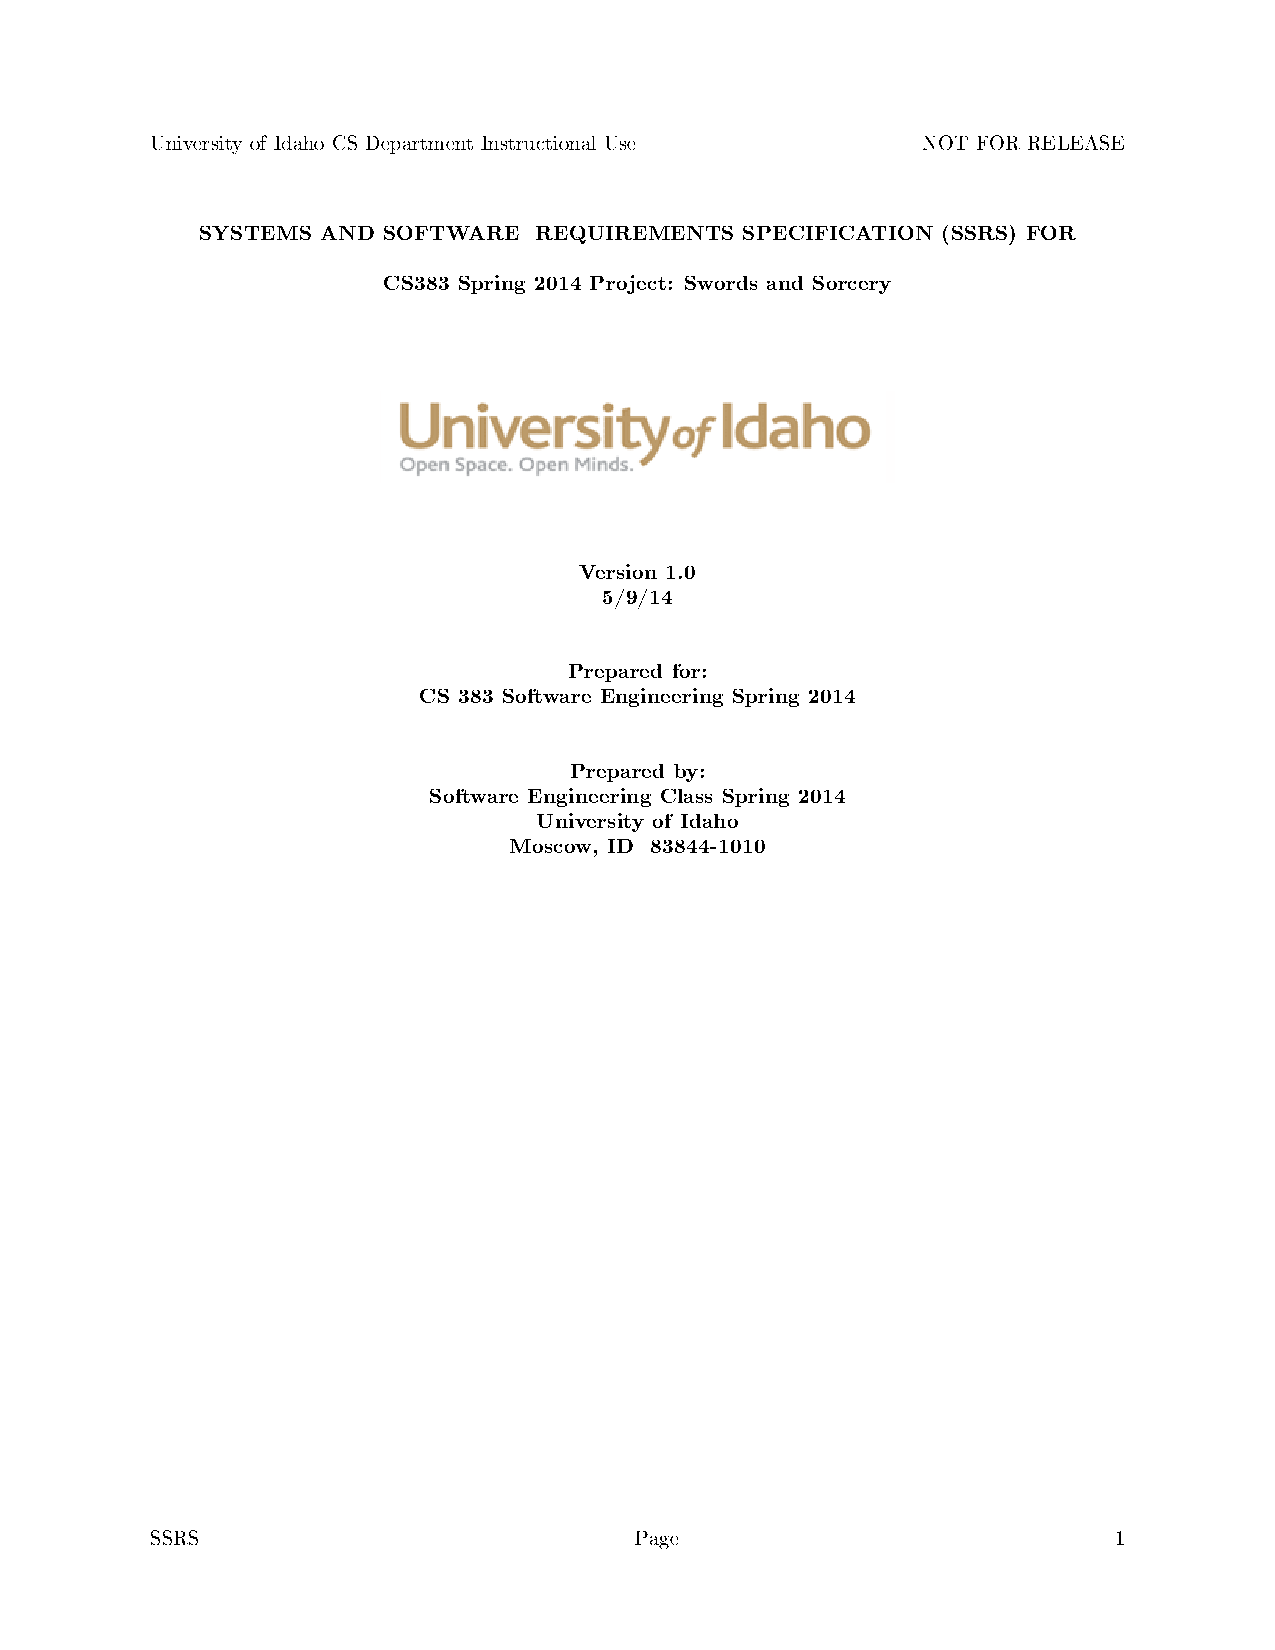
\includepdf[pages=-]{ssrs}

\includepdf[pages=-]{cs383SSDD}

\includepdf[pages=-]{Implementation}
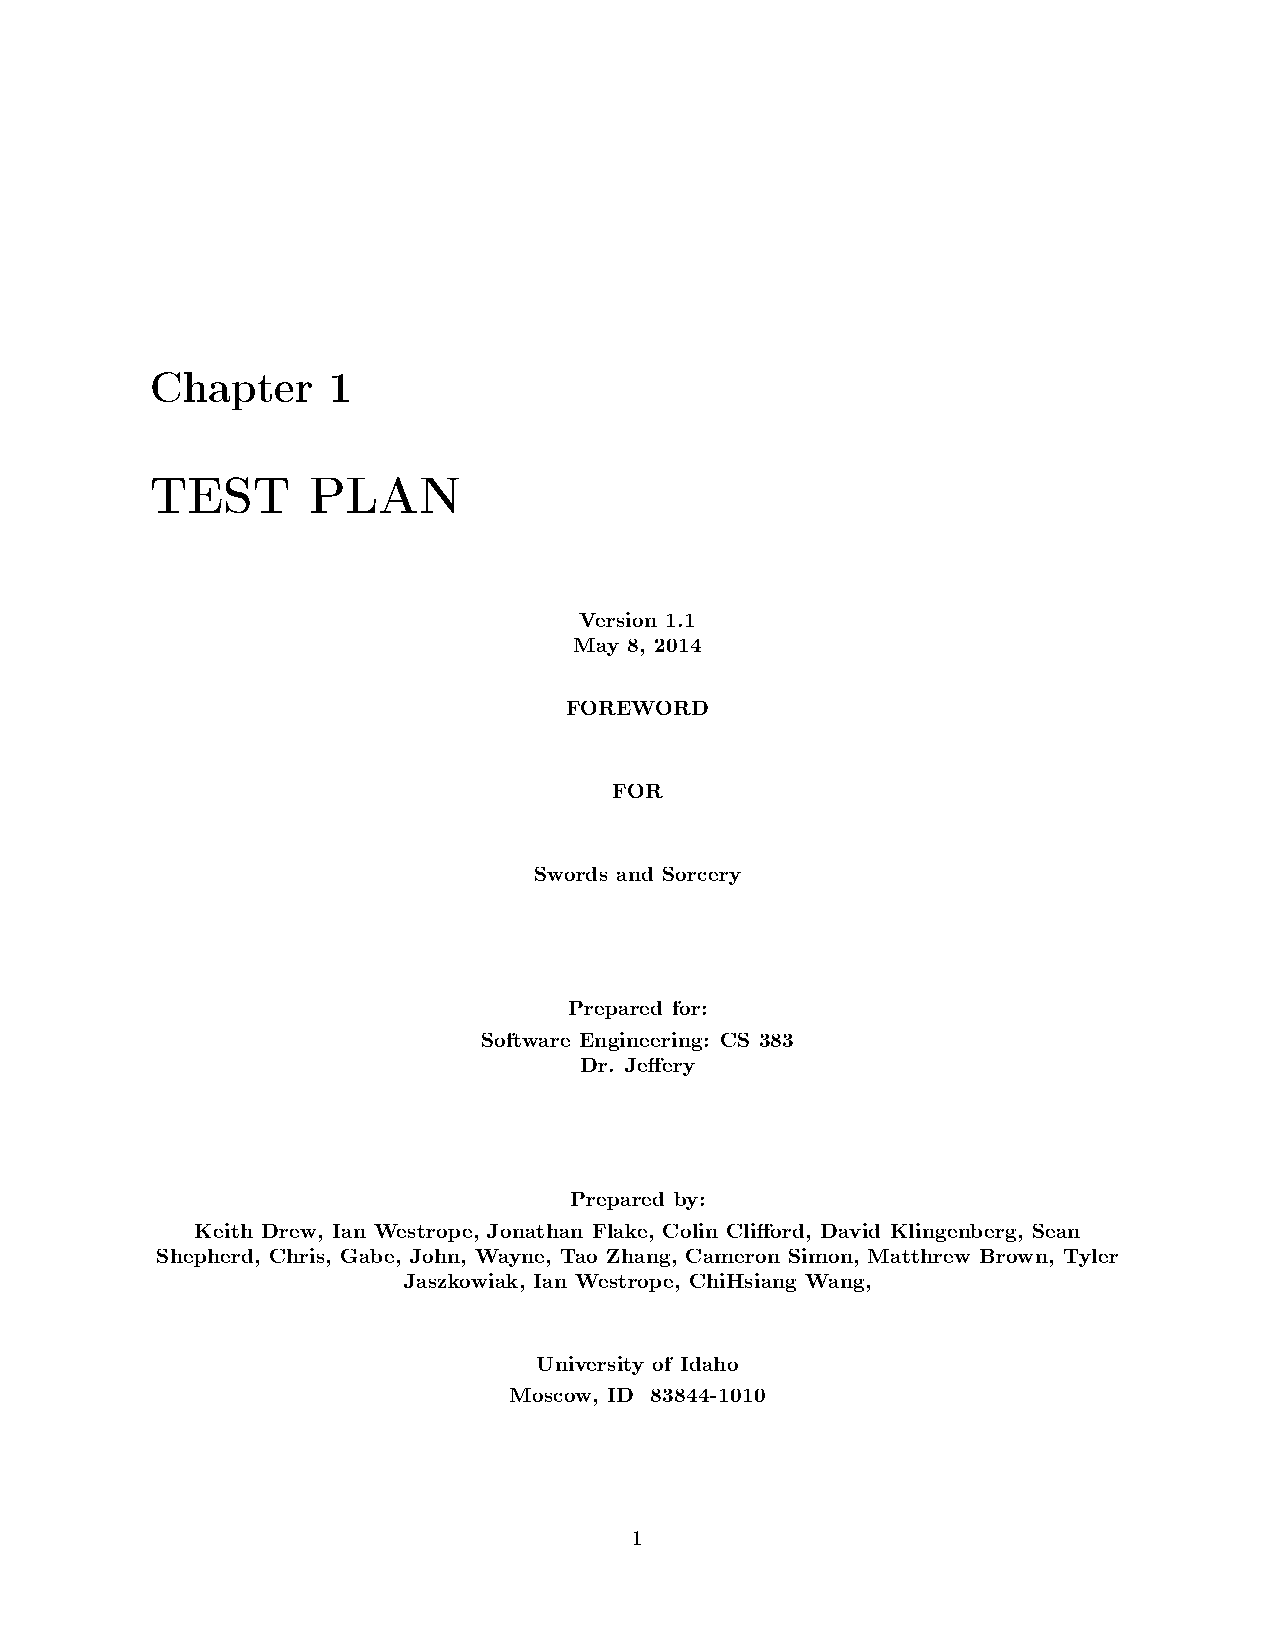
\includepdf[pages=-]{TP_Template}
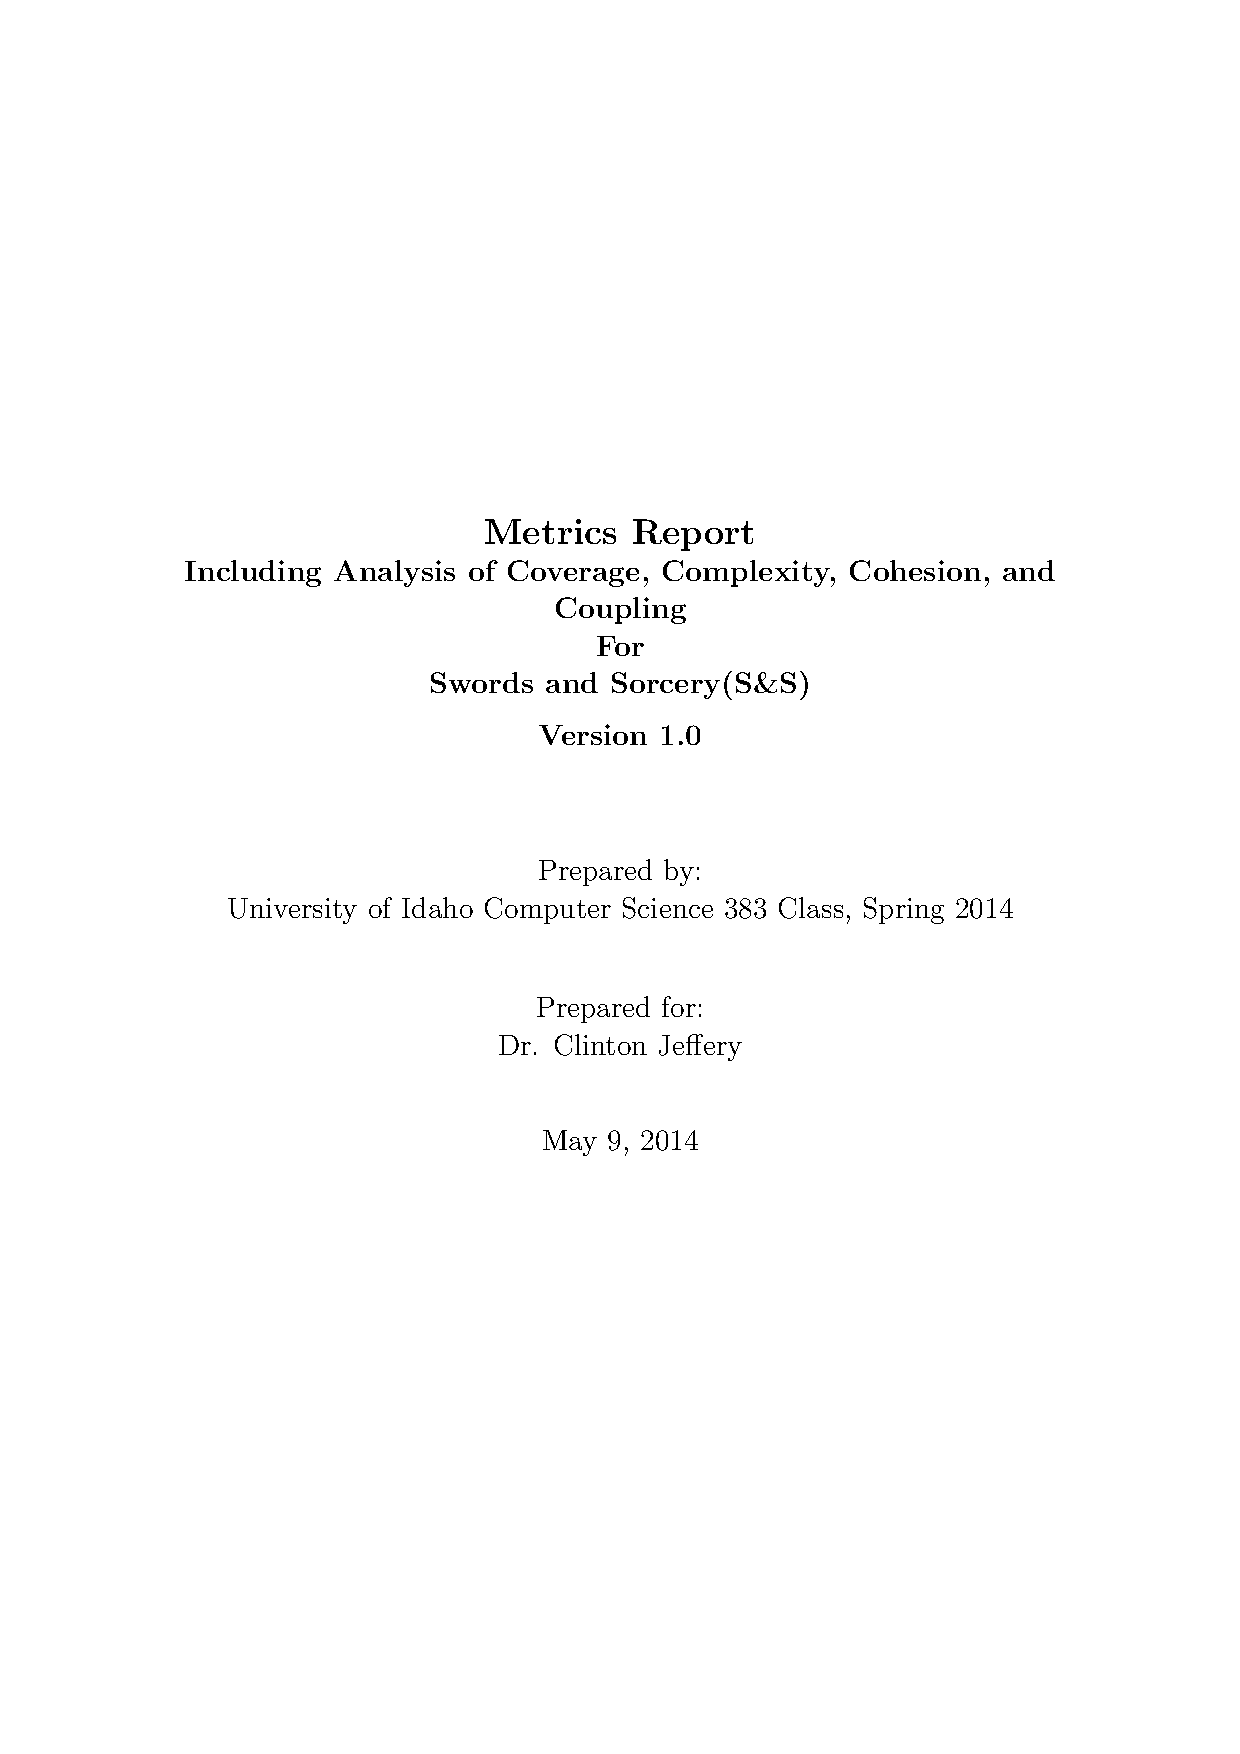
\includepdf[pages=-]{metrics_report}


\end{document}